\section{Etapa de memoria}
Una de las etapas mas simples del pipeline, se encarga de tomar los datos que provienen desde el latch y segun la senal activada, se encarga de leer o escribir en determinada posicion de memoria tambien suministrada.

\begin{figure}[H]
\centering
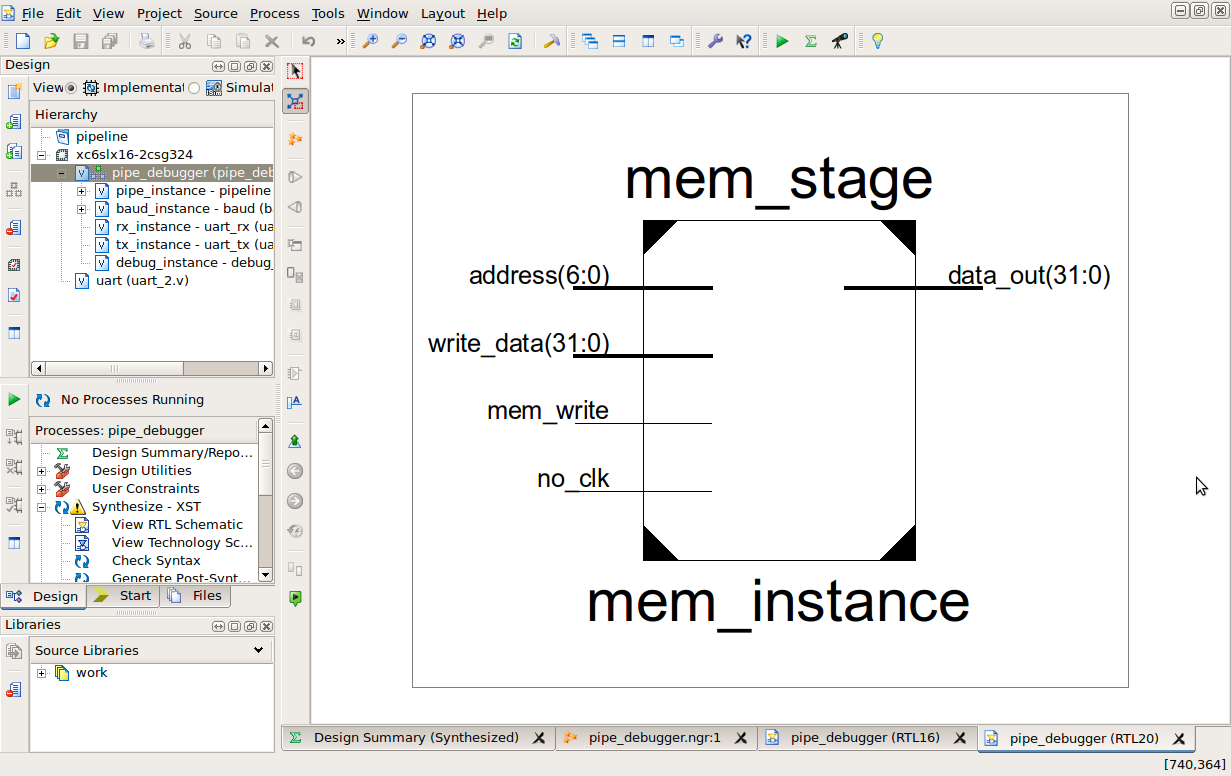
\includegraphics[scale=0.35]{img/mem_stage}
\caption{Etapa de memoria}
\label{fig:mem_stage}
\end{figure}

Tienen como entradas:
\begin{itemize}
  \item \textbf{address}:  Bus de 7 bits que indica a la memoria la direccion de la que se va a leer o escribir.
  \item  \textbf{write\_data}: Bus de 32 bits que contiene los datos que se van a escribir en la memoria.
  \item \textbf{mem\_write}: Senal que si esta en uno, se escribe en la memoria, si esta en cero, se lee.
  \item \textbf{no\_clk}: Reloj general del sistema. 
\end{itemize}

Salidas:

\begin{itemize}
  \item \textbf{data\_out}: Bus de 32 bits que contiene el dato que fue leido de la memoria.
\end{itemize}